\documentclass[11pt]{article}
\usepackage[margin=1in]{geometry}
\usepackage{amsmath,amssymb}
\usepackage{graphicx}
\usepackage{booktabs}
\usepackage{hyperref}
\usepackage[numbers,sort&compress]{natbib}

\title{How Few Spikes Are Enough?\\
       Sparse Event-Based Neuromorphic Decoding for Implantable BCI}
\author{Manraj Mondair \and Alexander Soto}
\date{EE207: Neuromorphics — Brains in Silicon}

\begin{document}
\maketitle

\begin{abstract}
Brain-computer interfaces (BCIs) must decode movement intent accurately,
quickly, and with very low power. Standard decoders convert spikes into
dense firing-rate vectors and apply classical machine learning, a
representation that is poorly matched to implantable devices where
computation, heat, memory movement, and wireless bandwidth are severely
constrained. We compare a standard spike-count ridge regression decoder
against a sparse spike-latency spiking neural network decoder on the
Neural Latents Benchmark MC\_RTT motor-cortex dataset, sweeping the
fraction~$f$ of earliest spike events processed per 50~ms bin and
measuring continuous 2D cursor-velocity~$R^2$. We add an order-shuffle
control to test whether within-bin spike order itself carries decoding
information.

\end{abstract}

\section{Introduction}
Implantable BCIs are a natural application area for neuromorphic
computing because the input signal is already event-like: neurons
communicate through sparse spikes. Standard decoding pipelines discard
this event structure by binning spikes into firing rates and processing
the resulting dense vectors with conventional machine learning. We
instead ask whether the input representation itself can be made more
neuromorphic --- can sparse spike timing and spike order support
continuous motor decoding under aggressive event budgets?

\section{Dataset}
We use the Neural Latents Benchmark MC\_RTT
dataset~\cite{nlb2021}: spiking activity from primary motor cortex
during a self-paced random-target reaching task, with simultaneously
recorded cursor position, finger position, and target position. The
decoding target is the continuous 2D cursor velocity
$v_t = (v_{x,t},\, v_{y,t})$, computed by centered finite differences
from the cursor position trace and resampled onto 50~ms bin centers.

We bin spikes into 50~ms windows, producing both a dense spike-count
matrix and a sparse per-bin event list of $(t_i, n_i)$ pairs --- spike
time within the bin and neuron identifier, sorted by time. The dense
view feeds the ridge baseline; the sparse view feeds the SNN. The
processed object is documented in \texttt{docs/data\_interface.md} and
both decoders depend on it as a fixed contract.

Splits are time-contiguous (first 70\% train, next 15\% validation,
last 15\% test) with one bin dropped on each side of every split
boundary so that finite-difference velocities cannot leak labels
across splits.

\section{Methods}

\subsection{Baseline: Spike-Count Ridge Regression}
For each bin~$t$ we form the spike-count vector
$x_t = [c_{1,t}, c_{2,t}, \ldots, c_{N,t}]$, where $c_{i,t}$ is the
number of spikes neuron~$i$ fires in window~$t$, and predict
$\hat v_t = W x_t + b$ via $L^2$-regularized linear regression. The
regularizer~$\alpha$ is selected on the validation split from a
log-spaced grid and the chosen value refit on the training split before
scoring on the held-out test split.

\subsection{Sparse Spike-Latency SNN (Alexander)}
\emph{Placeholder for SNN method description, written by the SNN-side
collaborator.}

\subsection{Event Budget}
The key experiment restricts how much neural information the decoder
processes. In each bin, spike events are sorted by time and only the
earliest fraction $f \in \{1.00, 0.50, 0.25, 0.10\}$ is retained. For
the ridge baseline, the spike-count vector is recomputed from the
retained events. For the SNN, only the retained events enter the
network.

\subsection{Order-Shuffle Control (Alexander)}
\emph{Placeholder for the within-bin order shuffle control, written by
the SNN-side collaborator.}

\section{Evaluation}

The primary decoding metric is joint velocity~$R^2$, summed over both
cursor velocity dimensions before division:
\[
R^2 = 1 - \frac{\sum_t \| v_t - \hat v_t \|_2^2}
                {\sum_t \| v_t - \bar v \|_2^2}.
\]
Per-axis $R^2_{v_x}$ and $R^2_{v_y}$ are reported alongside for
interpretability but the headline ranking uses the joint formula.

As a secondary efficiency variable we report the number of spike events
processed at each budget and the corresponding multiply-accumulate
(MAC) cost: dense ridge prediction performs $2N$ MACs per bin
($X \cdot W + b$ with $X \in \mathbb{R}^{1\times N}$,
$W \in \mathbb{R}^{N\times 2}$), while an event-driven implementation
of the same linear readout adds $W[n_i,:]$ into a running accumulator
on each retained spike (2~MACs per event) plus the bias add per bin.
\emph{MACs avoided} is the headline secondary number.

\section{Results}

\paragraph{Ridge baseline.} \emph{Placeholder: results table with
$R^2_{v_x}$, $R^2_{v_y}$, $R^2_{\text{joint}}$, and best~$\alpha$ at each
event budget, averaged across seeds.}

\paragraph{Sparse SNN.} \emph{Placeholder for SNN-side results.}

\paragraph{Order-shuffle control.} \emph{Placeholder for shuffle
control.}

\paragraph{Accuracy-efficiency frontier.}
The headline figure is $R^2_{\text{joint}}$ vs.\ event budget~$f$,
overlaying ridge, SNN, and shuffle curves
(Figure~\ref{fig:frontier}).

\begin{figure}[h]
  \centering
  % 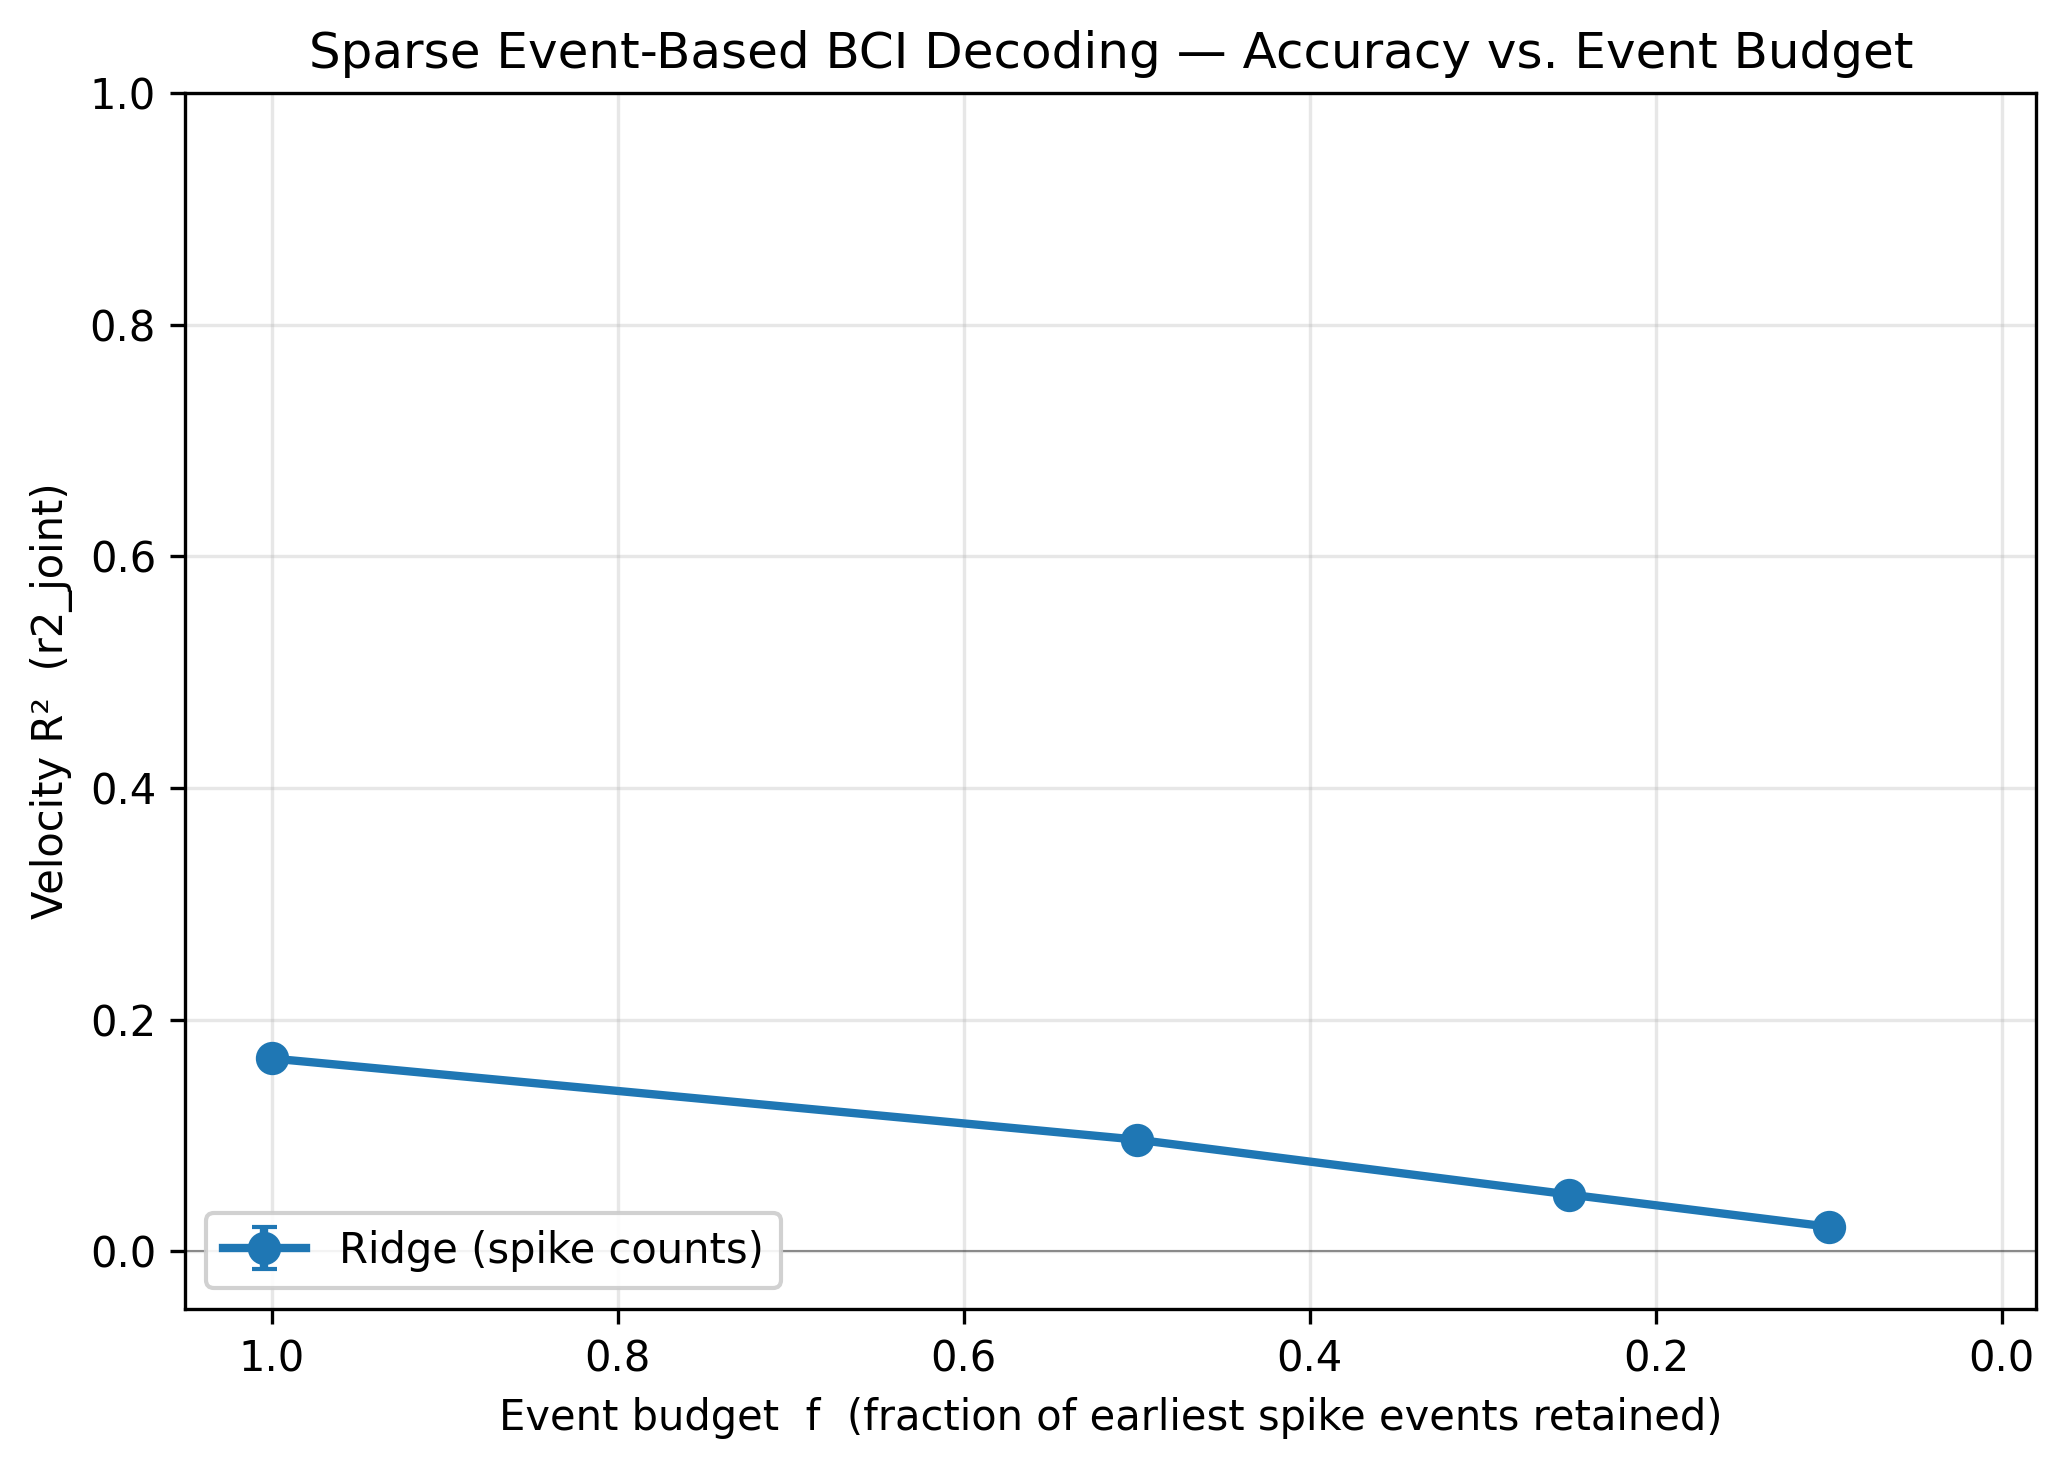
\includegraphics[width=0.85\linewidth]{../results/figures/accuracy_efficiency_frontier.png}
  \caption{Velocity $R^2$ vs.\ fraction of earliest spike events
  retained per bin. \emph{Placeholder --- to be replaced once all three
  models have produced canonical-schema JSON results.}}
  \label{fig:frontier}
\end{figure}

\paragraph{Secondary efficiency.}
\emph{Placeholder: events processed per budget and MACs avoided
relative to the dense baseline.}

\section{Discussion}
\emph{Placeholder: when does spike order help, when do counts win,
and how steeply does accuracy degrade with the event budget.}

\section{Class Alignment}
This project applies EE207's framing of spike patterns as latency
vectors and lookup-table transformations to a concrete neuromorphic BCI
problem. The central question --- whether useful movement intent can
be decoded from a sparse early-spike representation --- mirrors the
course's emphasis on spatiotemporal spike patterns, spike-latency
coding, and the energy cost of dense neural computation.

\bibliographystyle{plainnat}
\bibliography{refs}

\end{document}
